\documentclass[conference]{IEEEtran}
\IEEEoverridecommandlockouts
% The preceding line is only needed to identify funding in the first footnote. If that is unneeded, please comment it out.
\usepackage{cite}
\usepackage{amsmath,amssymb,amsfonts}
\usepackage{algorithmic}
\usepackage{graphicx}
\usepackage{textcomp}
\usepackage{xcolor}
\usepackage{multirow}
\def\BibTeX{{\rm B\kern-.05em{\sc i\kern-.025em b}\kern-.08em
    T\kern-.1667em\lower.7ex\hbox{E}\kern-.125emX}}
\begin{document}

\title{Numeric Methods Benchmark Analysis}

\author{\IEEEauthorblockN{1\textsuperscript{st} Santiago Valencia Arango}
\IEEEauthorblockA{\textit{dept. of science} \\
\textit{EAFIT}\\
Medellín, Colombia \\
svalenciaa@eafit.edu.co}
\and
\IEEEauthorblockN{2\textsuperscript{nd} Juan Manuel Young Hoyos}
\IEEEauthorblockA{\textit{dept. of science} \\
\textit{EAFIT}\\
Medellín, Colombia \\
jmyoungh@eafit.edu.co}
}

\maketitle

\begin{abstract}
The idea of this project is to test out if it is worth it to use C++ instead of Python for
algorithms of some numeric methods, like finding roots of non-linear equations using
Newton-Raphson's method.
\end{abstract}

\begin{IEEEkeywords}
Numeric methods, C++, Python, algorithms, insert
\end{IEEEkeywords}

\section{Introduction}
Why this project? the aim of this project is to be able to analyze and draw a conclusion to 
the question, is it worth spending more time programming in C ++? Or is it more profitable to do 
this type of algorithms using Python and its libraries in terms of development time and program performance?

\section{Objectives}
In this project we seek to compare the efficiency of developing root search methods in python against c++, taking into account the comparison between these two languages for this we looked for the implementation of these algorithms in both languages for further analysis taking into account the speed and memory consumption of these algorithms in each of the languages.

\section{Theoretical framework}

The purpose of calculating the roots of an equation is to determine the values of x for which the following is true 

\ 

\begin{equation}
 f(x)= 0
\end{equation}                                                    

\

The determination of the roots of an equation is one of the oldest problems in mathematics and a great number of efforts have been made in this direction. Its importance lies in the fact that if we can determine the roots of an equation we can also determine maxima and minima, eigenvalues of matrices, solve systems of linear and differential equations[2].

\ 

The determination of the solutions of equation (1) can become a very difficult problem. If f(x) is a polynomial function of degree 1 or 2, we know simple expressions that will allow us to determine its roots. For polynomials of degree 3 or 4 it is necessary to use complex and laborious methods. However, if f(x) is of degree greater than four or is not polynomial, there is no known formula that allows us to determine the zeros of the equation (except in very particular cases).[2]


For this we have resorted to the use of technological tools that allow the calculation of these roots in a much more efficient way than doing it by traditional methods, for that we are looking for the implementation of different algorithms that facilitate the search of these roots[2].



\ 

Python is a very popular interpreted language nowadays among people looking to work with data and mathematical functions due to its ease of use and the large number of libraries that exist, as well as its great ease of development compared to other languages such as c++ or java, one of the disadvantages of python is that its performance compared to compiled languages is usually lower. In python you can use extensions like cython that allow the use of libraries and compile the code looking to optimize it over the c++ compiler, this option would seek to improve the efficiency of this same[3].

\

C++ is widely used in general-purpose programming languages. The language allows you to encapsulates high and low-level language features. So, it is seen as an intermediate-level language. It also used to develop complex systems where the hardware level coding requires[4].


When comparing Python vs C++, Python follows a rule of “write once, run anywhere,” which means that one code will work on all operating systems. However, the C++ code needs to compile on each OS before it can execute.[5]

The biggest difference in the discussion of Python vs C++ is that the C++ source code needs to become machine code. Python follows a different tactic as it is interpreted. However, the interpretation of code is usually slower than running code directly on the hardware.[5]


\

\section{Algorithms}


\subsection{bisection}
The bisection method is a closed method of finding a solution of an equation of the form $ f(x) = 0 $ within a given interval $ [a, b] $ .

\


Algorithm:

\
1.Choose the first interval by finding the points $ a $ and $ b $ such that there is a solution between them. That is, that $ f(a) $ y $ f(b) $ thave different signs such that $ f(a) f(b) < 0 $.

\

2. Calculate the first estimate of the numerical solution: $$ m = \frac{a+b}{2} $$

\

3. This is done by checking the sign of the product $ f(a) \cdot f(m) $ :

\

    * If $ f(a) \cdot f(m) < 0 $, the real solution lies between $ x_{a} $ y $ m $

 \

    * If $ f(a) \cdot f(m > 0 $, the real solution lies between $ m $ y $ b $

\

4. Select a new subinterval that contains the true solution, either $ [a, m] $ o $ [m, b] $.

\

5. Steps 1 to 4 are repeated until a specified tolerance or error limit is reached.



\

\subsection{Regula falsi}

The false position or Regula Falsi method is a bracketed method for finding a numerical solution to an equation of the form $ f(x = 0 $ within a given interval $ [a, b] $ .
solution of an equation of the form $ f(x) = 0 $ within a given interval $ [a, b] $ .

In that interval, the equation of a straight line joining $ a$ and $ b $ is:


\begin{equation}
 y = \frac{f(b) - f(a)}{b - a} (x - b) + f(b)
\end{equation}

\

From (2), the point of $ m $ where the line intersects the x-axis is determined by substituting $ y = 0 $ and solving for $x$:

\

\begin{equation}
 m = \frac{a\cdot f(b) - b \cdot f(a)}{f(b) - f(a)}
\end{equation}

\

The procedure (or algorithm) for finding a solution with the regula falsi method is almost the same as that of the bisection method.


\


Algorithm:

\

1.Choose the first interval by finding the points $ a$ and $ b $ such that there is a solution between them. That is, let $ f(a) $ and $ f(b) $ have different signs such that $ f(a) f(b) < 0 $.

\

2.Calculate the first estimate of the numerical solution using (3)

\

3. Determine if the true solution is between $ a$ and $ m $, or between $ m $ and $ b $. This is done by checking the sign of the product $ f(a) \cdot f(m) $ :

\
    
	* If $ f(a) \cdot f(m) < 0 $, the real solution lies between $ a$ and $ m $

\

	* If $ f(a) \cdot f(m) > 0 $, the real solution lies between $ m $ and $ b $

\

4. Select a new subinterval that contains the true solution, either $ [a, m] $ or $ [m, b] $.

\

5. Steps 1 to 4 are repeated until a specified tolerance or error limit is reached.


\subsection{Fixed-point}

The fixed-point method finds a numerical solution of an equation of the form $ f(x) = 0 $ by rearranging the equation such that x is on the left-hand side:

\ 

\begin{equation}
 x =  g(x)
\end{equation}


\


\begin{equation}
 x_{i+1} =  g(x_{i})
\end{equation}

\



\subsection{Newton-Rapshon}

If the initial guess of the root is $ x_{i} $, a tangent/straight line can be extended from the point $ (x_{i}, f(x_{i})) $. The point where this tangent crosses the x-axis represents an improved estimate of the root.


\

The Newton-Raphson method can be derived from this geometric interpretation. The derivative at a point is:


\



\begin{equation}
 f^{'}(x_{i}) = \frac{f(x_{i+1}) - f(x_{i})}{x_{i+1} - x_{i}}
\end{equation}

\ 

Setting $ f(x_{i+1}) = 0 $, we obtain:


\


\begin{equation}
f^{'}(x_{i}) = \frac{0 - f(x_{i})}{x_{i+1} - x_{i}}
\end{equation}


\begin{equation}
x_{i+1} = x_{i} - \frac{f(x_{i})}{f^{'}(x_{i})}
\end{equation}


\


(1) is called the Newton-Rhapson formula and starts from an initial value, $ x_{0} $.


\ 


The method starts from an initial value, $ x_{0} $. It can be proven that convergence is quite likely when $ g^{'}(x) < |1| $ .

\

Although the Newton-Raphson method is usually very effective, 
there are situations in which it does not work well. Its convergence depends on the nature of the function and the accuracy of the initial estimate.

\


* If an inflection point ($ f^{''}(x) = 0 $) occurs near the root, the Newton-Raphson technique may oscillate around a local maximum or minimum.

\


* The worst-case scenario is an extremum ($ f^{'}(x) = 0 $) that causes a division by zero because the solution shoots horizontally and never reaches the x-axis.

\

The method starts from an initial value, $ x_{0} $. It can be proven that convergence is quite likely when $ g^{'}(x) < |1| $ .


\subsection{Secant}

One potential problem in the application of the Newton-Raphson method is the evaluation of the derivative. While this is not inconvenient for polynomials and many other functions, there are certain functions whose derivatives can be extremely difficult or inconvenient to evaluate. For these cases, the derivative can be approximated by a direct difference:


\


\begin{equation}
f^{'}(x_{i}) = \frac{f(x_{i+1}) - f(x_{i})}{x_{i+1} - x_{i}}
\end{equation}

\


Instead of using two values of x, the modified secant method introduces a small perturbation fraction, $ \delta$, such that (1) becomes:

\

\begin{equation}
f^{'}(x_{i}) = \frac{f(x_{i} + \delta x_{i}) - f(x_{i})}{\delta x_{i}}
\end{equation}

\

Substituting (10) in the Newton-Rhapson formula,


\

\begin{equation}
f^{'}(x_{i}) = \frac{f(x_{i} + \delta x_{i}) - f(x_{i})}{\delta x_{i}}
\end{equation}


\


The choice of a suitable value for $ °delta $ is not automatic. If $ \delta$ is too small, the method becomes vulnerable to rounding errors caused by subtractive cancellation in the denominator of (3). If it is too large, the technique can become inefficient and even divergent. However, if chosen correctly, it provides a good alternative for cases where the evaluation of the derivative is difficult and the development of two initial guesses is inconvenient.
\section{What will we test?}


\subsection{Algorithms}
In this project we will only find roots of an equation using:
\begin{itemize}
    \item Newton-Rapshon method.
    \item Bisection method.
    \item Secant method.
    \item Regula-Falsi method.
    \item Fixed-point iteration method.
\end{itemize}


\

The algorithms explained above were developed in python and c++, and will be tested to compare the efficiency of these in each of the cases, for this we will test different functions that seek to see the speed and resource consumption with which these methods are executed in each of the attempts.

\




\section{Procedures}


For the execution of the methods we looked for different functions that allow the comparison of these methods for this we will run each of the methods with the corresponding functions, and we will use the \textit{linux time} tool that allows us to measure how long it takes to run our programs.

\


To count the amount of time consumed by each of the tests, they were run with the linux time command, which allows us to know how long it takes to execute a process.


\


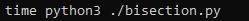
\includegraphics[width=5cm, height= 1cm]{com.PNG}


\

As you can see the execution time of a program, in this case the real time is the one that determines the execution time.

\


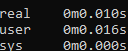
\includegraphics[width=4cm, height= 1cm]{con2.PNG}


\subsection{Bisection}

For the execution in both python and c++ the following parameters will be configured:

\

Equation: \(3x^3 - 2x -5\) 

Lower end: \(0\)

upper end: \(2\)

Tolerance: \(0.00001\) 

Maximum number of iterations: \(20\)



\subsection{Regula falsi}

For the execution in both python and c++ the following parameters will be configured:

\

Equation: \( \cos(x) - x e^x \) 

Lower end: \(0\)

upper end: \(2\)

Tolerance: \(0.00001\) 

Maximum number of iterations: \(20\)


\subsection{Fixed point}

For the execution in both python and c++ the following parameters will be configured:

\

Equation: \(\frac{2 - e^x + x^2}{3}\)

Initial point: \(0\)

Tolerance: \(0.00001\) 

Maximum number of iterations: \(20\)


\subsection{Newton Rapshon}

For the execution in both python and c++ the following parameters will be configured:

\

Equation: \( 3x^2  - 2x  \) 

Initial point: \(0\)

Tolerance: \(0.00001\) 

Maximum number of iterations: \(20\)



\subsection{Secant}

For the execution in both python and c++ the following parameters will be configured:

\ 

Equation: \(x^3 + 1\) 

Lower end: \(0\)

upper end: \(2\)

Tolerance: \(0.00001\) 

Maximum number of iterations: \(20\)



\subsection{machine}

Components with which each of the tests were carried out

\


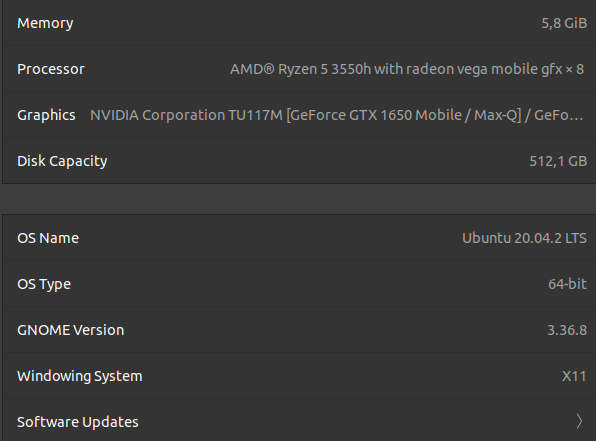
\includegraphics[width=8cm, height= 5cm]{specs2.PNG}







\section{Results}

\subsection{Bisection}

For the function, the method was run 10 times to observe the different changes in the method.

\


\begin{tabular}{|c|l|l}
\hline
\multicolumn{3}{|c|}{\(3x^3 - 2^x - 5\)}     \\ \hline
\# Results & \multicolumn{1}{c|}{Python} & \multicolumn{1}{c|}{C++}   \\ \hline
1          & \multicolumn{1}{c|}{0.229}  & \multicolumn{1}{c|}{0.104} \\ \hline
2          & \multicolumn{1}{c|}{0.206}  & \multicolumn{1}{c|}{0.012} \\ \hline
3          & 0.216                       & \multicolumn{1}{l|}{0.016} \\ \hline
4          & 0.207                       & \multicolumn{1}{l|}{0.021} \\ \hline
5          & 0.204                       & \multicolumn{1}{l|}{0.023} \\ \hline
6          & 0.208                       & \multicolumn{1}{l|}{0.017} \\ \hline
7          & 0.209                       & \multicolumn{1}{l|}{0.016} \\ \hline
8          & 0.204                       & \multicolumn{1}{l|}{0.023} \\ \hline
9          & \multicolumn{1}{c|}{0.207}  & \multicolumn{1}{c|}{0.022} \\ \hline
10         & \multicolumn{1}{c|}{0.205}  & \multicolumn{1}{c|}{0.023}  \\ \hline
\end{tabular}




\ 


From this, the average of these 10 executions is kept looking for the average execution time of the method, finding that the method executed with c++ is around 10 times more efficient than the one made in python.

\



\begin{tabular}{|c|c|c|}
\hline
\multicolumn{3}{|c|}{Average}              \\ \hline
\multirow{2}{*}{Results} & Python & C++    \\ \cline{2-3} 
                         & 0.2095 & 0.0187 \\ \hline
\end{tabular}




\ 


\subsection{Regula falsi}

For the function, the method was run 10 times to observe the different changes in the method.


\begin{tabular}{|c|c|c|}
\hline
\multicolumn{3}{|c|}{\(cos(x)  -  x * e^x\)} \\ \hline
\# Results               & Python              & C++                \\ \hline
1                        & 0.209               & 0.039              \\ \hline
2                        & 0.218               & 0.042              \\ \hline
3                        & 0.244               & 0.039              \\ \hline
4                        & 0.214               & 0.041              \\ \hline
5                        & 0.212               & 0.057              \\ \hline
6                        & 0.222               & 0.044              \\ \hline
7                        & 0.214               & 0.048              \\ \hline
8                        & 0.215               & 0.053              \\ \hline
9                        & 0.224               & 0.049              \\ \hline
10                       & 0.215               & 0.047              \\ \hline
\end{tabular}

\





From this, the average of these 10 executions is kept looking for the average execution time of the method, finding that the method executed with c++ is around 5 times more efficient than the one made in python.

\


\begin{tabular}{|c|c|c|}
\hline
\multicolumn{3}{|c|}{Average}             \\ \hline
\multirow{2}{*}{Results} & Python & C++   \\ \cline{2-3} 
                         & 0.216  & 0.045 \\ \hline
\end{tabular}




\subsection{Fixed-point}

\

For the function, the method was run 10 times to observe the different changes in the method.



\begin{tabular}{|c|l|l}
\hline
\multicolumn{3}{|c|}{\(2 - e^x + x ^2\)}     \\ \hline
\# Results & \multicolumn{1}{c|}{Python} & \multicolumn{1}{c|}{C++}   \\ \hline
1                        & 0.212               & \multicolumn{1}{c|}{0.031}              \\ \hline
2                        & 0.222               & \multicolumn{1}{c|}{0.044}              \\ \hline
3                        & 0.214               & \multicolumn{1}{c|}{0.042}              \\ \hline
4                        & 0.215               & \multicolumn{1}{c|}{0.041}              \\ \hline
5                        & 0.235               & \multicolumn{1}{c|}{0.052}              \\ \hline
6                        & 0.214               & \multicolumn{1}{c|}{0.043}              \\ \hline
7                        & 0.217               & \multicolumn{1}{c|}{0.041}              \\ \hline
8                        & 0.213               & \multicolumn{1}{c|}{0.034}              \\ \hline
9                        & 0.222               & \multicolumn{1}{c|}{0.058}              \\ \hline
10                       & 0.212               & \multicolumn{1}{c|}{0.051}              \\ \hline
\end{tabular}


\


From this, the average of these 10 executions is kept looking for the average execution time of the method, finding that the method executed with c++ is around 5 times more efficient than the one made in python.

\

\begin{tabular}{|c|c|c|}
\hline
\multicolumn{3}{|c|}{Average}              \\ \hline
\multirow{2}{*}{Results} & Python & C++    \\ \cline{2-3} 
                         & 0.2176 & 0.0437 \\ \hline
\end{tabular}




\subsection{Newton-Rapshon}


For the function, the method was run 10 times to observe the different changes in the method.

\

\begin{tabular}{|c|l|l}
\hline
\multicolumn{3}{|c|}{\(x^3 - x^2+ 2\)}   \\ \hline
\# Results & \multicolumn{1}{c|}{Python} & \multicolumn{1}{c|}{C++}   \\ \hline
1          & \multicolumn{1}{c|}{0.655}  & \multicolumn{1}{c|}{0.028} \\ \hline
2          & \multicolumn{1}{c|}{0.748}  & \multicolumn{1}{c|}{0.024} \\ \hline
3          & 0.717                       & \multicolumn{1}{l|}{0.019} \\ \hline
4          & 0.812                       & \multicolumn{1}{l|}{0.021} \\ \hline
5          & 0.697                       & \multicolumn{1}{l|}{0.017} \\ \hline
6          & 0.721                       & \multicolumn{1}{l|}{0.022} \\ \hline
7          & 0.694                       & \multicolumn{1}{l|}{0.023} \\ \hline
8          & 0.686                       & \multicolumn{1}{l|}{0.017} \\ \hline
9          & \multicolumn{1}{c|}{0.707}  & \multicolumn{1}{c|}{0.024} \\ \hline
10         & \multicolumn{1}{c|}{0.729}  & \multicolumn{1}{c|}{0.028} \\ \hline
\end{tabular}


\


From this we take the average of these 10 executions looking for the average execution time of the method, finding that the method executed with c++ is more or less 20 to 32 times more efficient than Python.


\

\begin{tabular}{|c|c|c|}
\hline
\multicolumn{3}{|c|}{Average}              \\ \hline
\multirow{2}{*}{Results} & Python & C++    \\ \cline{2-3} 
                         & 0.7166 & 0.0223 \\ \hline
\end{tabular}




\  



\subsection{Secant}



For the function, the method was run 10 times to observe the different changes in the method.


\





\begin{tabular}{|c|c|c|}
\hline
\multicolumn{3}{|c|}{\(x^3 + 1\)} \\ \hline
\# Results               & Python              & C++                \\ \hline
1                        & 0.777               & 0.011              \\ \hline
2                        & 0.735               & 0.012              \\ \hline
3                        & 0.682               & 0.010              \\ \hline
4                        & 0.680               & 0.011              \\ \hline
5                        & 0.705               & 0.010              \\ \hline
6                        & 0.670               & 0.011              \\ \hline
7                        & 0.690               & 0.010              \\ \hline
8                        & 0.670               & 0.011              \\ \hline
9                        & 0.680               & 0.012              \\ \hline
10                       & 0.673               & 0.010              \\ \hline
\end{tabular}


\



From this we take the average of these 10 executions looking for the average execution time of the method, finding that the method executed with c++ is more or less 50 times more efficient than the one made in python.

\



\begin{tabular}{|c|c|c|}
\hline
\multicolumn{3}{|c|}{Average}              \\ \hline
\multirow{2}{*}{Results} & Python & C++    \\ \cline{2-3} 
                         & 0.6962 & 0.0108 \\ \hline
\end{tabular}





\



\section{Conclusion}
In conclusion the construction of root equation methods in both python and c++ are relatively simple, the comparison was based on discovering the performance of these numerical methods in a interpreted language vs a compiled language, in this case the comparison between python and c++ gives us some pretty clear results, c++ is much more efficient executing the algorithms, and not constituting a very high development complexity with respect to python, because normally due to the convenience of the libraries in python usually the development of these methods are faster, but if you are looking for efficiency in the results should be developed with c++. 

\

With respect to the level of knowledge that you must have to develop these algorithms should be much higher in the case of c++, compared to python. 

\

A topic that was not treated in this project and that is raised as future work is the development of these methods in python but to use an extension of c++ that allows the execution of functions and declaration of variables with c++ allowing the facility of python and the great power of the compiler of c++ and its optimizations. 

\

\begin{thebibliography}{00}
\bibitem{b1} Burden, Richard L. and Faires, Duglas. Análisis Numérico. Editorial Thomson. 9 Edición 2011.
\bibitem{b2} Chapra, S. and Canale, R., 2003. Numerical methods for engineers. Boston: McGraw-Hill.
\bibitem{b3}L. Dalcin, et al.,"Cython: The Best of Both Worlds" in Computing in Science  Engineering, vol. 13, no. 02, pp. 31-39, 2011.doi: 10.1109/MCSE2010.118
\bibitem{4} A Brief Description - C++ Information", Cplusplus.com, 2021. [Online]. Available: https://www.cplusplus.com/info/description/.
\bibitem{5} Python vs C++ Comparison: Compare Python vs C++ Speed and More", BitDegree.org Online Learning Platforms, 2021. [Online]. Available: https://www.bitdegree.org/tutorials/python-vs-c-plus-plus/.
\end{thebibliography}

\end{document}
